% Chapter 3

\chapter{Implementation with OptiX} % Main chapter title here 

\label{Chapter3} % For referencing the chapter elsewhere, use \ref{Chapter3} 

\lhead{Chapter 3. \emph{Building with OptiX}} % This is for the header on each page perhaps a shortened title
\definecolor{mygreen}{rgb}{0,0.6,0}
\definecolor{mygray}{rgb}{0.9,0.9,0.9}
\definecolor{mymauve}{rgb}{0.58,0,0.82}
\definecolor{mybrown}{RGB}{178,34,34}

%\frametitle{Inserting source code without setting typewriter}
\lstset{language=C++,
  backgroundcolor=\color{mygray},
  numbers=left,                    % possible values are (none, left, right)
  numbersep=-8pt,                   % how far the line-numbers are from the code
  numberstyle=\tiny\color{mybrown}, % the style that is used for the line-numbers
  stepnumber=1,                    % each line will be numbered
  morekeywords={*,float3,Context,setRayTypeCount,setEntryPointCount,Material,
  launch,createProgramFromPTXFile,create,destroy,validate,compile,map,rtObject,
  setRayGenerationProgram,Program,setFloat,createBuffer,setElementSize,rtPrintf,
  Variable,Buffer,set,float4,rtDeclareVariable,rtBuffer,setBoundingBoxProgram,
  setIntersectionProgram,setPrimitiveCount,createGeometry,createMaterial,
  setClosestHitProgram,setGeometry,setMaterial,setMaterialCount,createGeometryInstance,
  GeometryInstance,GeometryGroup,createGeometryGroup,setChildCount,setChild,
  setAcceleration,createAcceleration,Ray,make_Ray,rtTrace,rtGetExceptionCode,
  rtIntersectionDistance,rtPayload,uint2,rtCurrentRay,attribute,
  Aabb,invalidate,createBufferForCUDA,cudaMalloc,set,setDevicePointer,
  rtPotentialIntersection,rtReportIntersection},
  keywordstyle=\color{blue},
  stringstyle=\color{mymauve},
  commentstyle=\color{mygreen},
  morecomment=[l][\color{magenta}]{\#},
  basicstyle=\footnotesize,        % the size of the fonts that are used for the code
  keepspaces=false,                 % keeps spaces in text, useful for keeping indentation of code
  columns=flexible,
  breaklines=true
  rulesepcolor=\color{mygray},
  rulecolor=\color{mygray}
}
%----------------------------------------------------------------------------------------

\section{OptiX Ray Tracing Basics}
\label{basics}
OptiX implementation consists of two major parts: a list of object-based models on the host and eight programs describing ray tracing specifics on the device. Host objects are in charge of establishing test scenes where take place all ray tracing algorithms. They assist in initializing geometries, passing data between host and device, launching OptiX kernels, handling post-treatments and so on. The combination of user-defined programs and built-in tracking algorithms forms the OptiX ray tracing control flow (\fref{fig:pipeline}).
%-------------------------------------------------------------------
\begin{figure}[htbp]
	\centering
		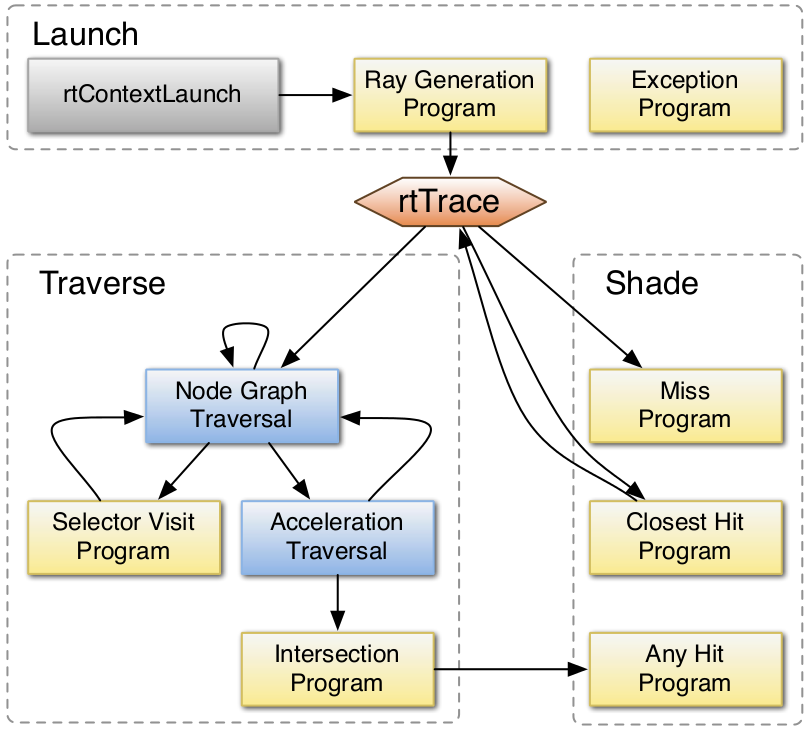
\includegraphics[width=9.5cm]{Figures/optixpipeline.png}
	\caption[The OptiX ray tracing pipeline]{The OptiX ray tracing pipeline \citep{Parker10OptiX}.}
	\label{fig:pipeline}
\end{figure}
%-------------------------------------------------------------------

Launching an OptiX kernel analogous to that of CUDA: after a ray tracing launch call (defined as \textit{rtContextLaunch} in OptiX) from CPU, all operations jump to the GPU side, where the first of the eight device programs, \textit{Ray Generation Program}, is automatically triggered. This first program initializes rays, their starting points and directions, and specifies the data that they carry. Once this is done, the tracking work begins. \textit{Bounding Box Program} accelerates tracking by reporting only potential primitives along a ray's trajectory. \textit{Intersection Program} allows all these geometries to record their crossing points with the ray and send this information to following \textit{Hit Programs}. \textit{Any Hit Program} is called every time a ray-object interface is found. Afterwards, among all the coordinates reported by \textit{Intersection Program}, OptiX will automatically point out the first intersection of each ray and call its corresponding \textit{Closest Hit Program}. It's in \textit{Closest Hit Program} that developers update ray information (direction, position and specific payload data) and continue tracing the new ray. For performance issue, any ray without potential intersections will be immediately killed after \textit{Intersection Program}. 

The main idea of ray tracing algorithms is representing ray propagations with a \textit{t} value. Any 2D or 3D coordinates will be transformed into this key word. For example, movement of a ray in the test scene is described as: 
\begin{equation}
	\vec{p} = \vec{o} + t\cdot\vec{d}
	\label{eq:1}
\end{equation}
Where $\vec{o}$ represents the origin of the ray and $\vec{d}$ represents its direction. A geometry primitive like sphere is the set of points at a given distance \textit{r} from a center point $\vec{c}$. It's easily expressed in vector form:
\begin{equation}
	(\vec{x} - \vec{c})^2 = r^2
	\label{eq:2}
\end{equation}
The equation of intersection points of the above ray and sphere can be substituted using \eref{eq:1} and \eref{eq:2}:
\begin{equation}
	(\vec{o} + t\vec{d} - \vec{c})^2 = r^2
\end{equation}
\begin{equation}
	(\vec{o} - \vec{c})^2 + 2t(\vec{o} - \vec{c})\cdot\vec{d} + t^2\cdot\vec{d}^2 = r^2
\end{equation}
As a result, the \textit{t} value: $t={\frac{-(2(\vec{o} - \vec{c})\cdot\vec{d})\pm\sqrt{(2(\vec{o} - \vec{c})\cdot\vec{d})^2-4((\vec{o} - \vec{c})^2-r^2)}}{2}}$.

%----------------------------------------------------------------------------------------
\section{Programming Model Overview}
As stated in the last section, OptiX programming model is constituted by the host code and the GPU device programs. This section gives an overview of these objects, programs and variables defined on CPU and executed on GPU. Note that models related to rendering concerns were not employed in our MC simulation, only the used ones will be presented and detailed in this report.

%----------------------------------------------------------------------------------------

\subsection{Host Models}
%------------------------------------
\begin{itemize}
  \item \textbf{Context:} The top object includes all other models in OptiX. Each \textit{Context} is an instance of the ray tracer.
  \item \textbf{Program:} An interface between user-defined codes and the eight OptiX device programs.
  \item \textbf{Variable:} A label used in communications between CPU and GPU. It must be bound to a \textit{Buffer}.
  \item \textbf{Buffer:} A multidimensional (host$\Leftrightarrow$device, CUDA$\Leftrightarrow$OptiX, OpenGL$\Leftrightarrow$OptiX, Direct3D$\Leftrightarrow$OptiX) array that transforms a \textit{Variable}.
  \item \textbf{Geometry:} Meshes or user-defined primitive that can be attached to multiple \textit{Materials} to handle multiple ray types (or interactions in MODERATO).
  \item \textbf{Material:} A container of \textit{Any Hit Program} and \textit{Closest Hit Program} attached to a specified OptiX ray.
  \item \textbf{GeometryInstance:} A combination of \textit{Geometry} and \textit{Material} objects.
  \item \textbf{GeometryGroup:} A set of \textit{GeometryInstance} objects.
  \item \textbf{Acceleration:} A structure which is bound to a \textit{GeometryGroup} and provides automatic accelerations.
\end{itemize}
%------------------------------------
Further information on these objects will be detailed in \sref{host}.
%----------------------------------------------------------------------------------------

\subsection{Device Programs}
%------------------------------------
\begin{itemize}
  \item \textbf{Ray Generation Program:} The entry point into the device-side ray tracing pipeline; where the radiation source in MODERATO is modeled.
  \item \textbf{Exception Program:} Program triggered while stack overflow or other errors, employed only for debug.
  \item \textbf{Closest Hit Program:} Handle calculations at the nearest intersection point, invoked by our MODERATO implementation to update cross-sections, create and trace new photons, etc.
  \item \textbf{Any Hit Program:} Called whenever a traced ray finds a new potential intersection point, unapplied in our implementation.
  \item \textbf{Intersection Program:} Where intersection detections take place, passing new free-path to Closest Hit Program in our implementation.
  \item \textbf{Bounding Box Program:} User-programmed bounding box, invoked during acceleration.
  \item \textbf{Miss Program:} Killing a traced ray when it misses all geometry primitives, unapplied in our implementation for performance concern.
\end{itemize}
%------------------------------------
\textit{PTX} is a virtual assembly language that can be easily interpreted by hardware architectures and requires no further compilation \citep{Reference2}. All OptiX \textit{Programs} must be compiled to \textit{.ptx} files in order to be combined with their host objects. These programs are further detailed in \sref{device}.
%----------------------------------------------------------------------------------------

\subsection{OptiX Ray Type}
OptiX \textit{Ray} is an encapsulation of a ray mathematical entity which is contained within the \textit{optix::} namespace. Except for some ray properties pre-defined within this object, every \textit{Ray} carries an user-defined \textit{rtRayPayload}. This payload contains variables we need for the following data processing. In our implementation of MODERATO, for example, it includes cross-section ratios, current free-path, photon energy, interaction counter, etc. Note that only an OptiX \textit{Ray} object can be accepted as an argument of \textit{rtTrace} function.

In order to take full advantages of pre-defined properties and avoid reloading them in a ray payload (which may degrade ray tracing performance), public attributes of OptiX \textit{Ray} are listed as follows:
\begin{lstlisting}[mathescape]
    /*	The origin of the ray; note that float3 is a CUDA	*  
     *	variable that corresponds to Vec3d in MODERATO.		*/
    float3 origin;
    
    float3 direction; // The direction of the ray
    
    unsigned int ray_type; // The ray type associated with this ray
    
    // The min and max extents associated with this ray
    float tmin;
    float tmax;
\end{lstlisting}

%----------------------------------------------------------------------------------------

\subsection{Internally Provided Semantics}
%----------------------------------------------------------------------------
\begin{figure}[htbp]
	%\centering 
		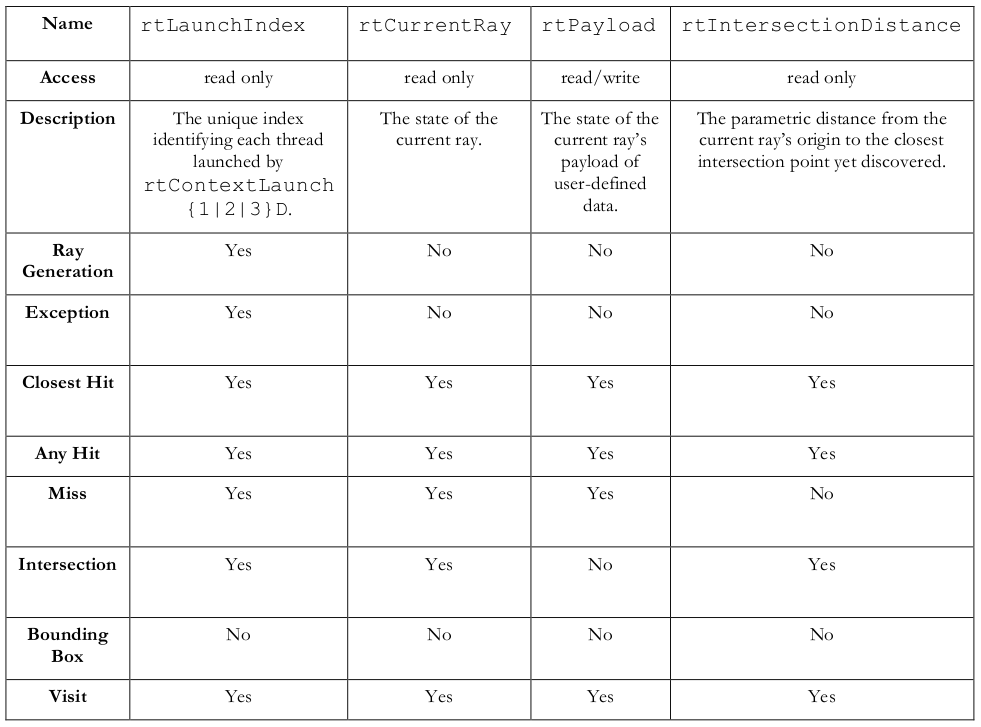
\includegraphics[width=\textwidth,height=\textheight,keepaspectratio]{Figures/semantics.png}
	\caption[Internal semantics provided by OptiX]{Internal semantics provided by OptiX \citep{Reference6}.}%
	\label{fig:semantics}
\end{figure}
%----------------------------------------------------------------------------
Certain variables can be frequently invoked by all eight OptiX programs. For example, a \textit{Ray} generated by \textit{Ray Generation Program} would be processed everywhere in the ray tracing pipeline: in \textit{Closest Hit Program} for changing direction, in \textit{Intersection Program} for finding potential interfaces, etc. Under the condition of large-scale parallelism, a global access to such variables without thread conflicts will be highly appreciated. To make it simple, OptiX manages several internal semantics for this program-variable binding. \fref{fig:semantics} summarizes in which types of program these semantics are available, along with their access rules from device programs \citep{optixref}.

%----------------------------------------------------------------------------------------

\section{Host Object Model}
\label{host}
Source code examples in either \textit{OptiX Programming Guide} or \textit{OptiX Quickstart Guide} only concern on C API of OptiX. As a result, in order to be familiar with the C++ wrapper and integrate OptiX in an existing object-oriented implementation, it's highly recommended to consult OptiX SDK and \textit{OptiX API Reference}. OptiX SDK provides various source code samples and is installed in the root directory by default.

%----------------------------------------------------------------------------------------

\subsection{Context}
\textit{Context} is the top node among the whole OptiX hierarchy. It encapsulates all resources for subsequent ray tracing control flows. Creation and destruction of this object are simple:
\begin{lstlisting}[mathescape]
    optix::Context context = Context::create();  // Setup context

    /* In MODERATO, we define that there are two types of rays. The first is normal ray, which models photons outside inspected objects. The second, called interaction ray, is responsible for representing photons that may change their energies, directions, free paths, etc.*/ 
    context$-$>setRayTypeCount( 2 );
    
    /* Indicate camera numbers in traditional ray tracing algorithms, here it figures the projection source number. We could therefore handle multi$-$source situation. */
    context$-$>setEntryPointCount( 1 );
    .........// a lot of codes...
    
    context$-$>destroy();  // Clean up and invalidate all resources 
\end{lstlisting}
OptiX kernel launch is realized by using \textit{Context}'s public member \textit{launch}. This host instruction starts the device ray tracing pipeline. The maximum kernel size varies according to GPU card's \href{http://docs.nvidia.com/cuda/cuda-c-programming-guide/index.html#compute-capabilities}{CUDA Compute Capability} as well as their memory size. Quadro FX 1800, a card with Capability 1.1, may afford 500$\times$500 launch indices. A 2.0 card like Quadro 5000, may increase up to 1000$\times$1000. The ceiling kernel size of each card is indicated nowhere in OptiX manual. Developers should explore it based on their own implementations.
\begin{lstlisting}[mathescape]
    ........  // Previous code, initializations...
    
    // Check the given context and all of its associated OptiX objects for a valid state and create final computation kernel from the given programs
    context$-$>validate();
    context$-$>compile();
    
    /* Launch a width*height OptiX kernel for source "0" (only one source). */
    context$-$>launch( 0, width, height );
    
    ......... // Collecting GPU data, post process...
\end{lstlisting}
Needless to say, even 1000$\times$1000 kernel is not big enough to simulate trillions of photons at the same time. We can use \textit{for} loop to achieve this purpose. Note that GPU computation has time-out concerns, simulations with a great number (billions or more, depends on the card) of photons require loops on both CPU and GPU side:
\begin{lstlisting}[mathescape]
    /* Launch a 1000*1000 OptiX kernel for 1000 iterations: a trillion photons created */
    for(i=0;i<1000;i++){   
      context$-$>launch( 0, 1000, 1000 );
\end{lstlisting}
%----------------------------------------------------------------------------------------

\subsection{Program}
\textit{Program} object is created from the \textit{.ptx} file. For instance, a \textit{Ray Generation Program} is defined in a CUDA file named \textit{ray.cu}.
\begin{lstlisting}[mathescape]
    RT_PROGRAM void ray_gen(){
      for(i=0;i<N;i++){   
        ... // cast photons....
      }
    }
\end{lstlisting}
After compiling \textit{ray.cu} into \textit{ray.ptx}, in the C++ main function, we establish the combination between host \textit{Program} object and device program \textit{ray\_gen} by calling \textit{createProgramFromPTXFile}.
\begin{lstlisting}[mathescape]
    // Set PTX file path
    std::string ptx_path( ptxPath( "ray" ) );
    
    // create host object "ray_gen_program" with device program "ray_gen"
    optix::Program ray_gen_program = context->createProgramFromPTXFile( ptx_path, "ray_gen" );
    
    // void optix::ContextObj::setRayGenerationProgram ( unsigned int entry_point_index, Program program )
    context$-$>setRayGenerationProgram( 0, ray_gen_program );
\end{lstlisting}

%----------------------------------------------------------------------------------------

\subsection{Variable and Buffer}
OptiX \textit{Variable} and \textit{Buffer} pass data between the host and the device. Communication of general variable types has been encapsulated within context's [ ] operator. In particular, transmission of tables or other special variable types will be implemented in another way:
\begin{lstlisting}[mathescape]
    // General types transfered by using [ ] operator
    context["ThetaMax"]$-$>setFloat( 4.f * 3.14159f/180 );
    context["O_source"]$-$>setFloat( 0.0f, 0.0f, 55.f );
    context["sphere"]$-$>setFloat( 0.f, 0.f, 0.f, 50.f );
    
    optix::Variable output = context["output"]; // a 1D table
    // A 1D table with 15 user-format elements
    optix::Buffer output_buffer = context$-$>createBuffer( RT_BUFFER_INPUT_OUTPUT, RT_FORMAT_USER, 15 );
    // User-format: unsigned long long int
    output_buffer$-$>setElementSize(sizeof(unsigned long long int)); 
    // Warning: must be bound to a Buffer. 
    output$-$>set(output_buffer);

    ...... // Kernel launch, device calculation, etc...
        
    // Then, we use map to collect data from GPU
    void* o_data = output_buffer$-$>map();
    unsigned long long int* result = (unsigned long long int*) o_data;
\end{lstlisting}
Within CUDA files, these global variables are declared just after header files:
\begin{lstlisting}[mathescape]
    #include ....
    
    // Accessible to all Programs within the file
    rtDeclareVariable(float,			ThetaMax, , );
    rtDeclareVariable(float3,			O_source, , );
    rtDeclareVariable(float4,			sphere, , );
    rtBuffer<unsigned long long int, 1>		output_buffer;
\end{lstlisting}
%----------------------------------------------------------------------------------------

\subsection{Geometry}
A \textit{Geometry} offers an interface to combine geometry representation with the ray tracing mechanism. This host object just passes setup parameters to its corresponding device \textit{Intersection Program} and \textit{Bounding Box Program}. It's only on the device that we describe geometry primitives and determine potential intersection points.
\begin{lstlisting}[mathescape]
    // Search device programs in the "object.ptx" (compiled from "object.cu") file
    std::string ptx_path( ptxPath( "object" ) );
    Geometry sphere = context$-$>createGeometry();
    // There is only one sphere in our case
    sphere$-$>setPrimitiveCount( 1u );
    
    // Set bounding box with the program named "bounds" in the "object.ptx"
    sphere$-$>setBoundingBoxProgram(context$-$>createProgramFromPTXFile(ptx_path,"bounds"));
    // "intersect" program establishes sphere description and intersection
    sphere$-$>setIntersectionProgram(context$-$>createProgramFromPTXFile(ptx_path,"intersect"));

    // Sphere parameter: origin (0,0,0) and radius=50
    sphere["sphere"]$-$>setFloat( 0.f, 0.f, 0.f, 50.f );
\end{lstlisting}

%----------------------------------------------------------------------------------------

\subsection{Material}
A \textit{Material} encapsulates the actions when a photon intersects a primitive or reaches the end of its current free-path. Two types of \textit{Hit Programs} can be assigned to a \textit{Material}, but only \textit{Closest Hit Program} is employed in our implementation. It is important to note that \textit{Hit Programs} are bound to \textit{Materials} per ray type, which means each \textit{Material} can actually hold more than one \textit{Closest Hit Program} \cite{Reference6}.
\begin{lstlisting}[mathescape]
    // Hit Program is situated in "object.ptx"
    std::string ptx_path( ptxPath( "object" ) );
    Material matl = context$-$>createMaterial();
    Program ch = context$-$>createProgramFromPTXFile( ptx_path, "closest_hit" );
    /* The Hit Program corresponds to ray type 0 (normal ray), more programs can be held:
     * matl$-$>setClosestHitProgram( 1, ch1 );
     * matl$-$>setClosestHitProgram( 2, ch2 ); */
    matl$-$>setClosestHitProgram( 0, ch );
\end{lstlisting}

%----------------------------------------------------------------------------------------

\subsection{GeometryInstance}
A \textit{GeometryInstance} represents a coupling of a single \textit{Geometry} with a set of \textit{Materials}. Note that multiple geometry instances are allowed to refer to a single geometry object, enabling a geometric object with different materials. Likewise, materials can be reused between different geometry instances.
\begin{lstlisting}[mathescape]
    // Create object with 1 geometry and 2 materials
    GeometryInstance object = context$-$>createGeometryInstance(); 
    object$-$>setGeometry( sphere );

    object$-$>setMaterialCount( 2 );
    // One material corresponds to the normal ray
    object$-$>setMaterial( 0, sphere_matl );
    // Another for interaction ray
    object$-$>setMaterial( 1, interaction_matl );
\end{lstlisting}

%----------------------------------------------------------------------------------------

\subsection{GeometryGroup}
A \textit{GeometryGroup} contains all \textit{GeometryInstances} in a test scene. In our first test MODERATO, for example, it represents a collection of an inspected sphere-object and a detector in parallelogram:
\begin{lstlisting}[mathescape]
    // Place all in geometry group
    GeometryGroup geometrygroup = context$-$>createGeometryGroup();
    geometrygroup$-$>setChildCount( 2 );
    // object and detector are GeometryInstances defined before
    geometrygroup$-$>setChild( 0, object );
    geometrygroup$-$>setChild( 1, detector );
\end{lstlisting}

%----------------------------------------------------------------------------------------

\subsection{Acceleration}
\textit{Acceleration} structures are important for speeding up the ray tracing process. Generally speaking, they decompose the hierarchical scene geometries into several basic boxes and cull non-intersection regions of space at the very beginning of the trace. The traversal is therefore accelerated by querying less geometries.

There are many different types of acceleration structures, each with their own advantages and drawbacks (\aref{AppendixB}). Note that no single type of acceleration structure is optimal for all scenes, it's developers themselves who find the best choice for their own implementations. Comparison among different structures for MODERATO test will be discussed in \sref{acc}.
\begin{lstlisting}[mathescape]
    /* Set acceleration with a "Bvh" builder and a "BvhCompact" traverser.
     * More details on introduction of OptiX acceleration structures see AppendixB */
    geometrygroup$-$>setAcceleration( context$-$>createAcceleration("Bvh","BvhCompact") );
\end{lstlisting}

%----------------------------------------------------------------------------------------
\section{Device OptiX Programs}
\label{device}
%----------------------------------------------------------------------------------------

\subsection{Ray Generation Program}
The following example implements a simple ray generation model. Each ray is generated by host-defined origin and direction with tmin=scene\_epsilon, tmax=RT\_DEFAULT\_MAX. The nature of these rays is "normal\_ray". Then, the user-defined payload will be charged with several photon characteristics: energy, diffusion counter, cross-section, etc. \textit{rtTrace} initialize the trace with a coupling of one ray and one payload.
\begin{lstlisting}[mathescape]
    // A user defined payload
    struct Photon{
      float3 S;			//S1, S2, S3
      float  energy;		// Photon energy
      int    nDiffusions;	// Diffusion counter
      ...
    };
    
    // Variables passed from the host side
    rtDeclareVariable(unsigned int,	normal_ray, , );
    rtDeclareVariable(float,		scene_epsilon, , );
    rtDeclareVariable(float3,		ray_origin, , );
    rtDeclareVariable(float3,		ray_direction, , );
    rtDeclareVariable(rtObject,		top_object, , );
    
    RT_PROGRAM void ray_gen(){   
      optix::Ray ray = optix::make_Ray(ray_origin, ray_direction, normal_ray, scene_epsilon, RT_DEFAULT_MAX);
      
      Photon payload;
      payload.energy = 1.f;
      payload.nDiffusions = 0;
      ...
      rtTrace(top_object, ray, payload);
    }
\end{lstlisting}
%----------------------------------------------------------------------------------------

\subsection{Exception Program}
\textit{Exception Program} is invoked when OptiX kernel encounters errors. The information provided by this program would be useful for debug. So as to have better tracing performance, however, it can be removed after application development.
\begin{lstlisting}[mathescape]
    rtDeclareVariable(uint2, launch_index, rtLaunchIndex, );
    
    RT_PROGRAM void exception()
    {
      const unsigned int code = rtGetExceptionCode();
      rtPrintf( "Caught exception 0x%X at launch index (%d,%d)\n", code, launch_index.x, launch_index.y );
    }
\end{lstlisting}

%----------------------------------------------------------------------------------------

\subsection{Closest Hit Program}
\textit{Closest Hit Program} is in charge of updating photon properties in our MODERATO implementation. Only in this program can we launch new rays (which means update randomly free-path, direction, interaction types, energy, etc.) and trace it.
\begin{lstlisting}[mathescape]
    rtDeclareVariable(float, t_hit,	rtIntersectionDistance, );
    rtDeclareVariable(Photon,  pd,	rtPayload, );
    
    RT_PROGRAM void closest_hit(){
      // Determine intersection point and change direction
      float3 hit_point = ray.origin + t_hit * ray.direction;
      new_direction = make_float3...

      pd.energy...  // Other updates

      // Launch a new ray at hit point and trace it
      optix::Ray new_ray(hit_point, new_direction, normal_type, scene_epsilon, RT_DEFAULT_MAX);
      rtTrace(top_object, new_ray, pd);
    }
\end{lstlisting}

%----------------------------------------------------------------------------------------

\subsection{Any Hit Program}
An \textit{Any Hit Program} is called wherever ray tracer finds an intersection point. It's necessary to point out that for all intersections along a cast ray, \textit{Any Hit Program} corresponding to each intersection point won't be invoked in order. In MODERATO, it's expected to find nearest intersection point, take update actions and launch the new ray. Unfortunately, \textit{Any Hit Program} matches none of these features because \textit{rtTrace} is only available in \textit{Ray Generation Program} and \textit{Closest Hit Program}. Furthermore, disabling useless programs contributes to better computing performance. Consequently, this program was not applied in our implementation.

However, \textit{Any Hit Program} could be very practical for the 2D1D neutronic simulation, where neutrons traversing geometries without changing direction or other properties in each intersection point are expected to be recorded. The problem of intersection sort will come into focus in this situation.

%----------------------------------------------------------------------------------------

\subsection{Intersection Program}
Code examples of a sphere \textit{Intersection Program} are presented in this sub-section. They demonstrate how to build a simple analytic geometry and query its ray-object intersections. 

Once the intersection program has determined the \textit{t} value of a ray-primitive intersection, it must report the result by calling a pair of OptiX functions, \textit{rtPotentialIntersection} and \textit{rtReportIntersection}. Note that another semantic, \textit{attribute}, is employed in this program. It's used to pass variables from \textit{Intersection Program} to \textit{Hit Programs}. Attrbute variables can only be written in \textit{Intersection Program} and only be placed between these two functions. In the example below, \textit{attribute distance} will be sent to \textit{Closest Hit Programs} for signalizing photons' traverse distance within sphere: 
\begin{lstlisting}[mathescape]
    rtDeclareVariable( float4,		sphere, , );
    rtDeclareVariable( optix::Ray, ray,	rtCurrentRay, );
    rtDeclareVariable( float, distance,	attribute distance, );

    // Intersection for sphere geometry
    RT_PROGRAM void intersect(int primIdx){
      float3 center = make_float3(sphere);
      float3 O = ray.origin $-$ center;
      float3 D = ray.direction;
      float radius = sphere.w;

      // analytic sphere solution
      // float a = dot(D, D); useless since direction is normalized, a=1
      float b = 2*dot(O, D);
      float c = dot(O, O)$-$radius*radius;
      float disc = b*b$-$4*c;

     // If there are two different intersections, we ignore the case with only one intersection
     if( disc > 0 ){
        float sdisc = sqrtf(disc);
        float tmin = ($-$b $-$ sdisc)/2;
        float tmax = ($-$b + sdisc)/2;

        // tmin will be surely nearest potential point, so we report it
        if( rtPotentialIntersection(tmin) ) {
          // Attribute data between rtPotentialIntersection and rtReportIntersection
          distance = (tmax $-$ tmin);
          // Call closest hit
          rtReportIntersection(0);
        } 
      } // if( disc >= 0 )
    } // intersection program
\end{lstlisting}
%----------------------------------------------------------------------------------------

\subsection{Bounding Box Program}
A \textit{Bounding Box Program} describes the minimal three dimensional axis-aligned cube that contains the geometry. The idea is to find out a primitive's minimum and maximum value in each dimension and create two points with three maximums and three minimums respectively. A cube formed by these two vertices is therefore the geometry's bounding box. We take an example of a sphere primitive:
\begin{lstlisting}[mathescape]
    rtDeclareVariable( float4, sphere, , );
    
    // Bounding box for sphere geometry
    RT_PROGRAM void bounds (int, float result[6])
    {
      const float3 cen = make_float3( sphere );
      const float3 rad = make_float3( sphere.w );

      // Axis-aligned bounding box
      optix::Aabb* aabb = (optix::Aabb*)result;
  
      if( rad.x > 0.0f  && !isinf(rad.x) ) {
        // first vertex with three minimums
        aabb$-$>m_min = cen $-$ rad;
        // second vertex with three maximums
        aabb$-$>m_max = cen + rad;
      } else {
        aabb$-$>invalidate();
      }
    }
\end{lstlisting}
%----------------------------------------------------------------------------------------

\section{CURAND: RNG on GPUs }
The CURAND library provides efficient pseudo-random and quasi-random number generators on GPUs. It's a RNG (Random Number Generator) API extremely optimized for GPU environment. According to the development group, the latest CURAND 6.0 performs up to 75x more powerful than Intel MKL \citep{cuda6report} (\fref{fig:curandmkl}).
%-------------------------------------------------------------------
\begin{figure}[htbp]
	\centering
		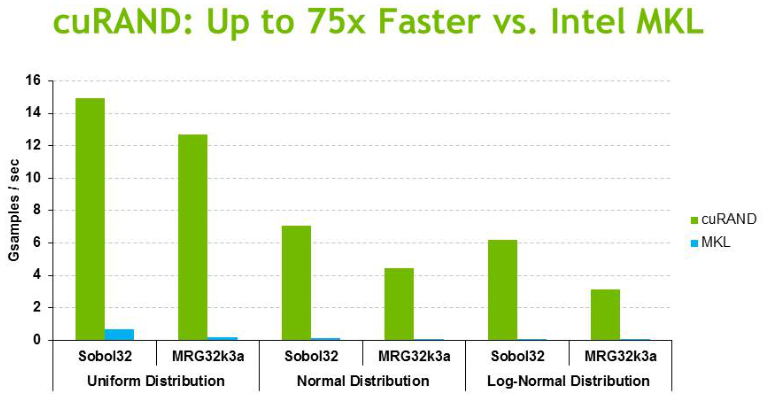
\includegraphics[width=13cm]{Figures/curand1.png}
	\caption[CURAND vs. MKL]{CURAND vs. MKL \citep{cuda6report}.}%
	\label{fig:curandmkl}
\end{figure}

CURAND encapsulates several popular PRNGs. Regardless of their difference on statistical properties, the standard XORWOW has the best performance (\fref{fig:curand}). Another PRNG highly recommended by developers is MRG32K3A. This generator preserves good statistic quality as well as satisfied performance. The most famous Mersenne Twister MTGP32 is widely used for scientific computing at present. Even if it maintains an impressively long period, its relatively poor efficiency on GPUs should always be taken into considerations for performance concerns. These three generators will be evaluated for our MODERATO implementation in the following of this section.
\vspace{1cm}
%-------------------------------------------------------------------
\begin{figure}[htbp]
	\centering
		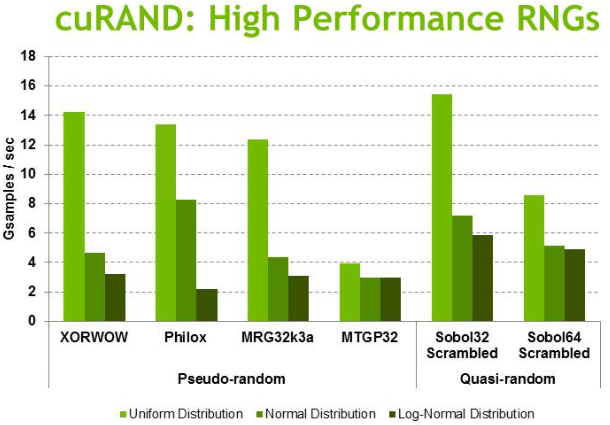
\includegraphics[width=13cm]{Figures/curand2.png}
	\caption[CURAND high performance RNGs]{CURAND high performance RNGs \citep{cuda6report}.}%
	\label{fig:curand}
\end{figure}
%-------------------------------------------------------------------

%----------------------------------------------------------------------------------------

\subsection{Mersenne Twister: MTGP32}
Mersenne Twister (MT) is one of the most widely used PRNG at the moment \citep{marsland2011machine}. MTGP32 is its variant optimized for GPUs. Just like the standard MT19937, MTGP32 has a very long period of $2^{19937}-1$, but it appears to be its only advantage.

The major drawback is that MTGP32 is fairly slow compared to other PRNGs: nearly three times more sluggish than other generators (\fref{fig:curand}). Moreover, it requires a very large state (624 words), which makes it memory-expensive if you want a random number sequence for each thread where you have tens of thousands of threads. Furthermore, these states heavily stress the GPU cache as well. MT's statistical property bring it grand reputation, however, it doesn't manage to pass all tests of TestU01 (Empirical statistical testing of uniform random number generators by L'Ecuyer) \citep{lecuyer}. 

As for an initial state with many zeros, MTGP32 will spend a long time on turning the state into output that passes randomness tests. \fref{fig:manyzeros} shows a test presented by L'Ecuyer: he initializes the state with a single bit at 1. The mean of uniform random outputs is badly deviated until 700000 iterations. Any developers who try to use MT in their implementations should pay attention to this issue.
%-------------------------------------------------------------------
\begin{figure}[htbp]
	\centering
		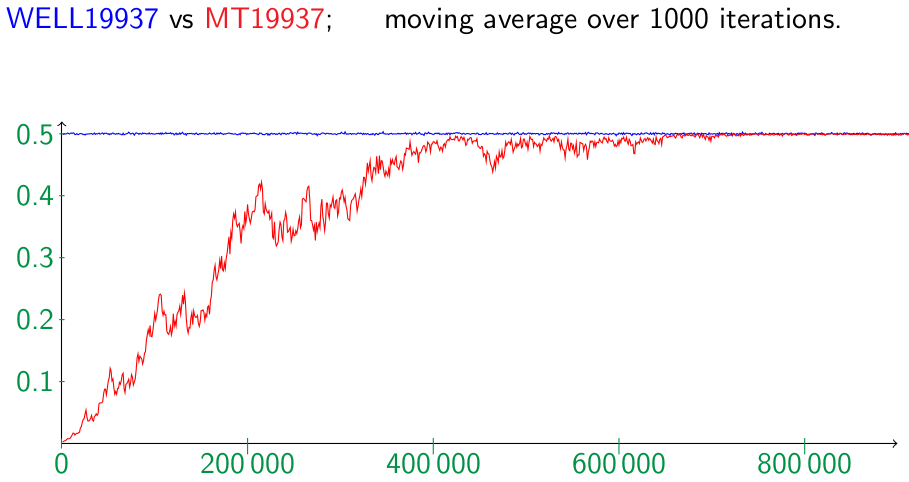
\includegraphics[width=13cm]{Figures/manyzeros.png}
	\caption[Initial state with a single bit at 1]{Initial state with a single bit at 1 \citep{lecuyer}.}
	\label{fig:manyzeros}
\end{figure}
%-------------------------------------------------------------------

Another point mentioned by CURAND tutorial is that MTGP32 is closely tied to the thread and block count and the most efficient use of MTGP32 is to generate a multiple of 16384 samples \citep{curand}. Unfortunately, OptiX has no thread control; the number of block is automatically distributed and optimized by the API. Hence MTGP32 might be neither safe nor efficient in OptiX. In conclusion, MTGP32 is not an efficient choice for our OptiX implementation.

%----------------------------------------------------------------------------------------

\subsection{Combined Multiple Recursive RNG: MRG32K3A}
MRG32K3A is a combined multiple-recursive generator with a period of $2^{191}$ \citep{l1999good}. It performs slightly slower than the fastest XORWOW (\fref{fig:curand}). However, it's one of the few generators recommended by L'Ecuyer since it passes all TestU01 randomness tests \cite{lecuyer}. 

An initial OptiX implementation was tested with this RNG. The result was not conclusive: output number sequences from different threads would produce repeatedly a certain value. This may signalize that different threads share a same state and MRG32K3A is sensitive to thread-safety. Debug of OptiX can be rather difficult for any problems related to thread control and the bug hasn't been solved yet.

%----------------------------------------------------------------------------------------

\subsection{XOR-Shift RNG: XORWOW}
XORWOW is the default generator type in CURAND with a period of $2^{192}-2^{32}$. It rapidly produces random numbers with efficient xor-shift operations, which contributes to its competitive performance against other RNGs. L'Ecuyer figured out that XORWOW is rejected by TestU01 \citep{l1999good}. Saito and Matsumoto conducted a deeper investigation to explain this rejection \citep{xorwow} and found that XORWOW has a significant deviation on 6-dimensional distribution of the most significant 5 bits. It means that one may find a particular regularity between a sixth random number and its previous five ones and therefore it's not strictly stochastic. At last, they concluded that this RNG is not ideal for serious Monte Carlo simulation.

The current OptiX implementation employs this RNG. Test results demonstrate that XORWOW preserve satisfied statistical characteristics since the difference between OptiX and the original code is negligible ($\approx$ $\pm$ 0.2\%, see \sref{optixperform}). Nevertheless, explorations of MRG32K3A would be taken into account in future work for serious simulations.

%----------------------------------------------------------------------------------------

\section{Interoperability with CUDA}
\label{interop}
It is often advisable to combine CUDA kernels with OptiX programs so that we can take full advantage of GPU performance. In our implementation, for instance, a CUDA kernel launched before OptiX content is responsible for initializing and seeding the CURAND RNG. Furthermore, other applications may request post-treatment of OptiX's output with CUDA. Both of these two cases require a CUDA-OptiX communication.

There are two possible solutions for this interoperability. One is to ask OptiX to allocate device memory and get a pointer to data. Another is to create OptiX buffers in CUDA kernels. The first method can be used for either feeding OptiX with data or postprocessing outputs. The second one, on the contrary, can be only used for pre-calculations since OptiX will neither allocate memory nor upload data for these buffers \citep{Reference6}. But this solution is similar to transferring data with \textit{Variable} and \textit{Buffer} that are used before and therefore easier to implement. In addition, its one-way communication capability has already satisfied initialization need. So we choose the second solution in MODERATO.

The use of CUDA buffers is nearly the same as normal host-device buffers:
\begin{lstlisting}[mathescape]
    optix::Variable states_buffer = context["states_buffer"];
      
    // Create an OptiX buffer for CUDA kernel         
    optix::Buffer states = context$-$>createBufferForCUDA( RT_BUFFER_INPUT, RT_FORMAT_USER, N );
    states$-$>setElementSize( sizeof(curandState) );
      
    // Allocate space for prng states on device 
    cudaMalloc((void **)&devStates, N * sizeof(curandState));
     
    // State setup is complete
    // Initialize one state per thread
    setup_kernel<<<h, w>>>(devStates, w);

    // Providing a device pointer for the CUDA$-$OptiX buffer
    states$-$>setDevicePointer( 0, reinterpret_cast<CUdeviceptr>(devStates) );
      
    // Attach buffer with the corresponding variable in OptiX Program
    states_buffer$-$>set(states);
\end{lstlisting}
Consult \textit{OptiX Programming Guide} for more details on getting CUDA device pointers from OptiX.
%----------------------------------------------------------------------------------------

\section{Performance Guidelines}
In terms of OptiX performance, several precautions should be taken in order to improve ray tracing process. Even small changes in the code can dramatically alter performance. Here is a list of some essential points based on OptiX manual, developers may complete it according to their own investigations \citep{Reference6}:
\begin{itemize}
  \item Use floats instead of doubles since float are already sufficient for MODERATO. This also extends to the use of literals and math functions. For example, use \textit{0.5f} instead of \textit{0.5} and \textit{sinf} instead of \textit{sin} to prevent automatic type promotion. 
  \item Compile PTX with \textit{-use-fast-math} option, it can reduce code size and increase the performance for most OptiX programs with a small decrease on accuracy. Replace standard functions with intrinsic functions when small accuracy errors are acceptable.
  \item Each new \textit{Program} object can introduce execution divergence. Try to reuse the same program with different variable values. For example, interaction rays and normal rays in MODERATO share the same sphere \textit{Intersection Program}.
  \item Minimize payload size and try to use a structure of arrays instead of an array of structures data. Any uninitialized variables can increase register pressure and degrade performance.
  \item Disable useless \textit{Programs} wherever possible: \textit{Miss}, \textit{Exception} and \textit{Any Hit Program} are disabled in the MODERATO implementation.
  \item Multiple access to global memory can be replaced by declaring local variables with much lower communication latency.
  \item No recursion on GPUs: tremendous complexity, try to replace it by iterations.
\end{itemize}
%----------------------------------------------------------------------------------------

\section{Programming Caveats}
OptiX hasn't been fully developed at the moment. Hence certain errors or bugs might appear during implementation. Even if this is a CUDA based API, it's not completely compatible with all CUDA features. Following caveats should be always kept in mind to avoid unnecessary mistakes \citep{Reference6}:
\begin{itemize}
  \item Setting a large kernel size will consume GPU device memory. Try to minimize the stack as much as possible. Start with a small stack and with the use of an exception program that indicates you have exceeded your memory, increase the stack size until the stack is sufficiently large. This is why a 1000$\times$1000 launch was available on Quadro 5000 but not on Quadro FX 1800, since the latter has smaller memory space.
  \item \_\_shared\_\_ memory within OptiX \textit{Programs} is forbidden.
  \item NEVER call CUDA \textit{syncthreads()} in OptiX Programs.
  \item CUDA threadIdx can map to multiple launch indices in OptiX. Use of OptiX \textit{rtLaunchIndex} semantic is mandatory.
  \item Currently, OptiX is not guaranteed to be thread-safe. OptiX should therefore be used only from a single host thread.
  \item Dynamic allocations are allowed in CUDA with 2.0 cards or greater \citep{cudaguide}, but not in OptiX Programs. Attempts to use these functions will result in an illegal symbol error.
\end{itemize}

%----------------------------------------------------------------------------------------
